\documentclass{article}
\usepackage{geometry}
\usepackage{amsmath}
\usepackage{graphicx}
\usepackage{hyperref}

\title{Application for Transcribing Grand Piano Recordings to Sheet Music in PDF}
\author{Michał Jagoda}
\date{\today}

\begin{document}

\maketitle

\tableofcontents

\section{Topic Analysis}

\subsection{Overview}
This project involves creating a desktop application designed to transcribe grand piano recordings into sheet music and export the results as a PDF. This involves the use of audio processing, music transcription, and PDF generation technologies, all performed locally without the need for an internet connection.

\subsection{Objectives}
\begin{itemize}
    \item To accurately transcribe piano recordings into readable sheet music.
    \item To provide a user-friendly interface for uploading audio files and exporting sheet music.
    \item To offer an offline and local application for accessibility and privacy reasons.
\end{itemize}

\subsection{Key Components}
\begin{itemize}
    \item \textbf{Audio Processing:} Capturing and processing the audio signals from the grand piano recordings using the \texttt{audio\_processor.py}.
    \item \textbf{AI Model:} Generating an initial transcription output from the uploaded MP3 file using the \texttt{transcription\_worker.py}.
    \item \textbf{Postprocessing Algorithm:} Creating a MIDI file from the AI model's output using the \texttt{Sheet\_music\_generation.py}.
    \item \textbf{PDF Generation:} Using the MuseScore API to generate a PDF from the generated MIDI file with \texttt{generate\_pdf.py}.
    \item \textbf{User Interface:} Allowing users to interact with the application, upload audio files, view PDF previews, listen to MIDI and MP3 files, and download the resulting sheet music and MIDI files via \texttt{window.py}.
\end{itemize}

\section{Technologies Used}
\begin{itemize}
    \item \textbf{Python:} The primary programming language used for developing the application.
    \item \textbf{Librosa:} A Python library for audio and music analysis, used for audio processing and feature extraction in \texttt{audio\_processor.py}.
    \item \textbf{Piano Transcription Inference:} A library for transcribing piano music, used in \texttt{transcription\_worker.py}.
    \item \textbf{Music21:} A toolkit for computer-aided musicology, used in \texttt{Sheet\_music\_generation.py} to create and manipulate music streams.
    \item \textbf{MuseScore:} A software for creating, playing, and printing sheet music, used in \texttt{generate\_pdf.py} to convert MIDI files to PDF.
    \item \textbf{PySide6:} A set of Python bindings for Qt libraries, used for creating the graphical user interface in \texttt{window.py}.
    \item \textbf{VLC:} A media player used for playing audio and MIDI files within the application.
    \item \textbf{Pdf2image:} A library for converting PDF files to images, used in the GUI to display PDF previews.
    \item \textbf{Tempfile:} A Python module used for creating temporary files, ensuring that the application handles file operations efficiently and securely.
    \item \textbf{WSL2 (Windows Subsystem for Linux):} Used to run some Python libraries that were not available on Windows. As WSL2 lacks support for audio and GUI components, server bridges were implemented to facilitate communication between the audio processing and GUI components running in different environments.
\end{itemize}

\section{Functional Requirements}

\subsection{Core Functionalities}
\begin{itemize}
    \item \textbf{Audio File Upload:}
    \begin{itemize}
        \item Users can upload MP3 audio files.
    \end{itemize}
    \item \textbf{AI Model:}
    \begin{itemize}
        \item The system processes the uploaded audio using an AI model to generate an initial transcription.
    \end{itemize}
    \item \textbf{Postprocessing Algorithm:}
    \begin{itemize}
        \item The application converts the AI model's output into a MIDI file.
    \end{itemize}
    \item \textbf{PDF Generation:}
    \begin{itemize}
        \item The MuseScore API is used to convert the generated MIDI file into a PDF document.
    \end{itemize}
    \item \textbf{PDF Preview and Download:}
    \begin{itemize}
        \item Users can preview the PDF of the sheet music.
        \item Users can download the PDF and the MIDI file.
    \end{itemize}
    \item \textbf{Playback Feature:}
    \begin{itemize}
        \item Users can listen to the transcription by playing the MIDI file.
        \item Users can also listen to the original MP3 file.
    \end{itemize}
\end{itemize}

\section{Non-Functional Requirements}

\subsection{Performance Requirements}
\begin{itemize}
    \item \textbf{Speed:} The transcription process should be completed within a reasonable time frame (under 15 minutes for a 5-minute recording).
    \item \textbf{Accuracy:} The transcription should accurately reflect the notes, rhythms, and dynamics of the original recording with a high degree of precision (over 90\% accuracy).
\end{itemize}

\subsection{Usability Requirements}
\begin{itemize}
    \item \textbf{User Interface:} The interface should be intuitive and easy to navigate, even for users with limited technical skills.
\end{itemize}

\subsection{Compatibility Requirements}
\begin{itemize}
    \item \textbf{File Format Support:} The application should support common audio file formats and produce PDFs that are compatible with standard PDF readers.
\end{itemize}

\subsection{Maintainability Requirements}
\begin{itemize}
    \item \textbf{Modularity:} The application code should be modular to facilitate easy updates and maintenance.
    \item \textbf{Documentation:} Comprehensive documentation should be provided for developers to understand the codebase and contribute to its development.
\end{itemize}

\subsection{Scalability Requirements}
\begin{itemize}
    \item \textbf{Future Expansion:} The architecture should allow for easy addition of new features and functionalities.
\end{itemize}

\section{Use Case Diagram}
\begin{figure}[h!]
    \centering
    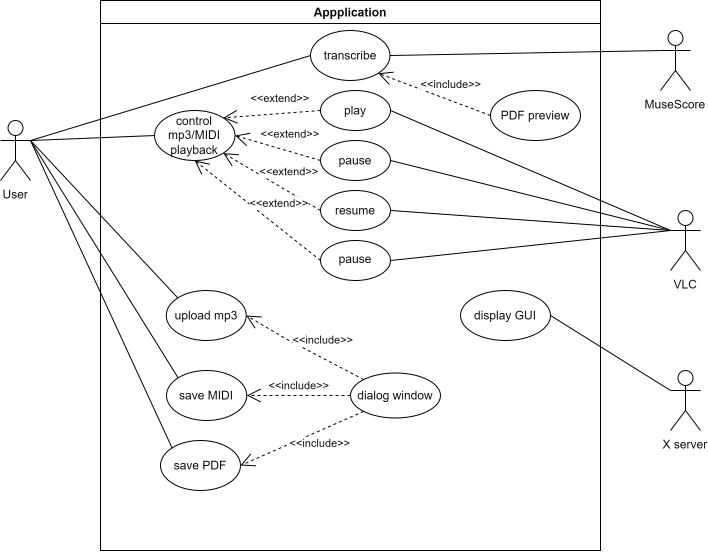
\includegraphics[width=0.8\textwidth]{../diagrams/use_case.png}
    \caption{Use Case Diagram}
    \label{fig:use_case}
\end{figure}

\section{System Architecture Flow Chart}
\begin{figure}[h!]
    \centering
    %\includegraphics[width=0.8\textwidth]{system_architecture_flow_chart.png}
    \caption{System Architecture Flow Chart}
    \label{fig:system_architecture}
\end{figure}

\section{Class Diagram}
\begin{figure}[h!]
    \centering
    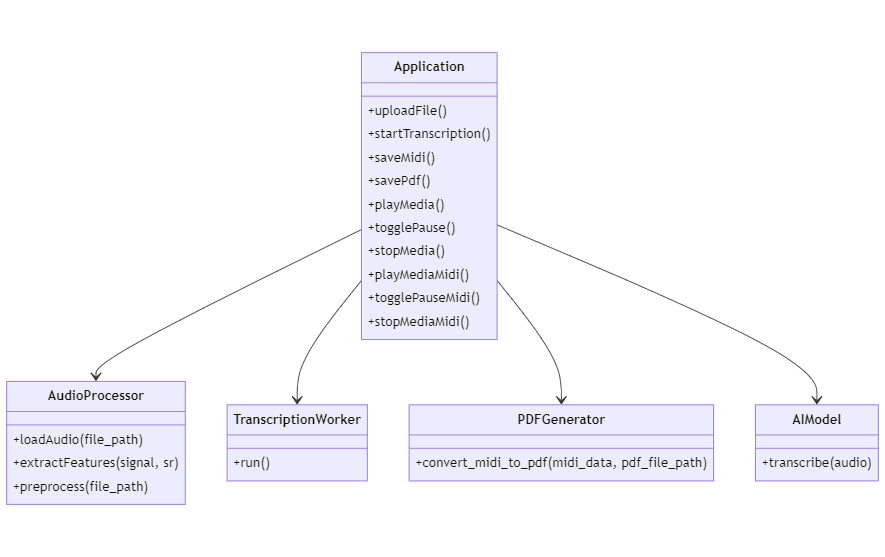
\includegraphics[width=0.8\textwidth]{../diagrams/class_diagram.png}
    \caption{Class Diagram}
    \label{fig:class_diagram}
\end{figure}

\section{Sequence Diagrams}

\begin{figure}[h!]
    \centering
    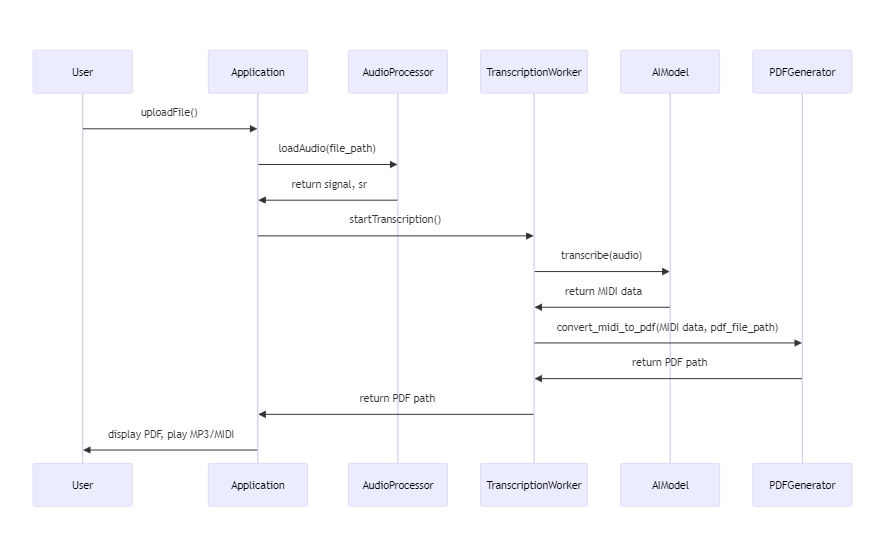
\includegraphics[width=0.8\textwidth]{../diagrams/transcription_seq.png}
    \caption{Transcription process sequence diagram}
    \label{fig:transcription_sequence_diagram}
\end{figure}

\begin{figure}[h!]
    \centering
    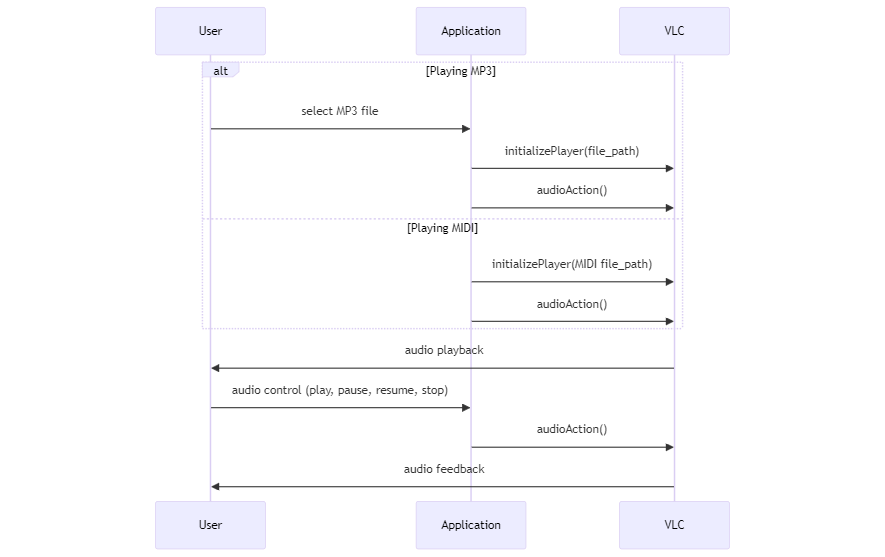
\includegraphics[width=0.8\textwidth]{../diagrams/audio_seq.png}
    \caption{Audio sequence diagram}
    \label{fig:audio_sequence_diagram}
\end{figure}

\begin{figure}[h!]
    \centering
    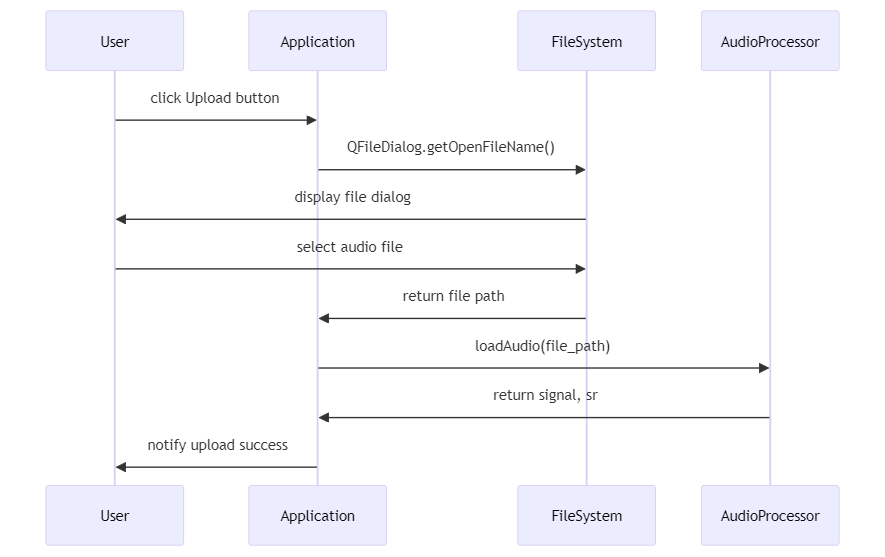
\includegraphics[width=0.8\textwidth]{../diagrams/load_audio_seq.png}
    \caption{Load file sequence diagram}
    \label{fig:load_audio_sequence_diagram}
\end{figure}

\begin{figure}[h!]
    \centering
    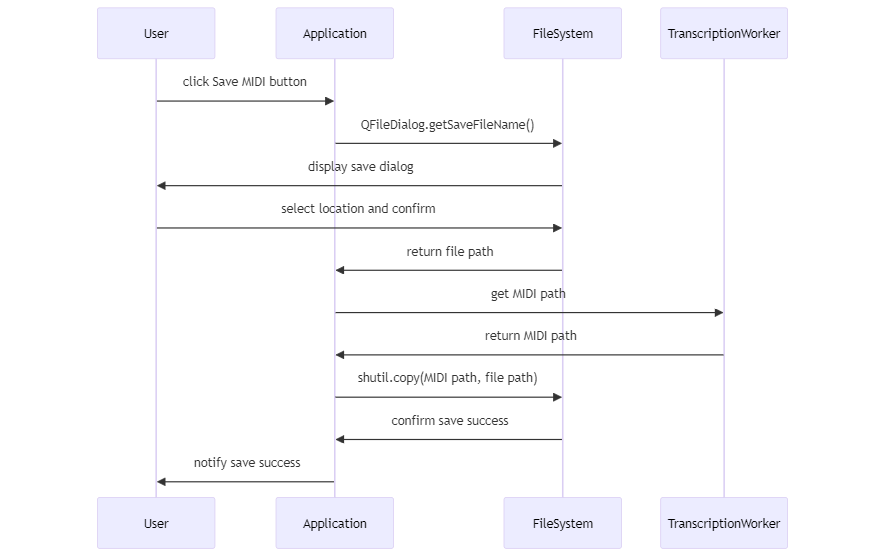
\includegraphics[width=0.8\textwidth]{../diagrams/save_midi_seq.png}
    \caption{Save MIDI sequence diagram}
    \label{fig:save_midi_sequence_diagram}
\end{figure}

\begin{figure}[h!]
    \centering
    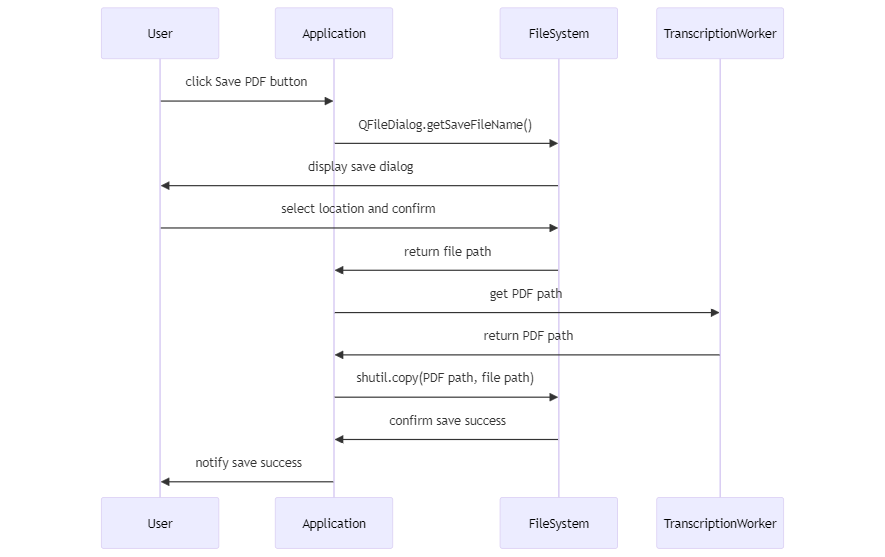
\includegraphics[width=0.8\textwidth]{../diagrams/save_pdf_seq.png}
    \caption{Save PDF sequence diagram}
    \label{fig:save_pdf_sequence_diagram}
\end{figure}


\section{AI Model Architecture}
\begin{figure}[h!]
    \centering
    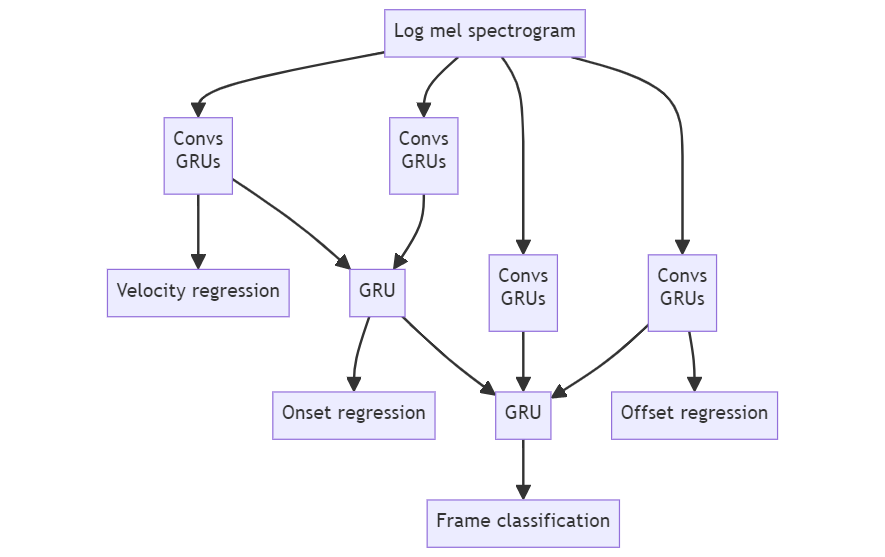
\includegraphics[width=0.8\textwidth]{../diagrams/ai_architecture.png}
    \caption{AI Model Architecture}
    \label{fig:ai_model_architecture}
\end{figure}

\section{Comparison of Original and Generated Sheet Music}
\begin{figure}[h!]
    \centering
    %\includegraphics[width=0.8\textwidth]{comparison_sheet_music.png}
    \caption{Comparison of Original and Generated Sheet Music}
    \label{fig:comparison_sheet_music}
\end{figure}

\section{Conclusion}
By addressing both the functional and non-functional requirements outlined above, this application can provide a robust, user-friendly solution for transcribing grand piano recordings into sheet music. This will not only meet the immediate needs of users but also ensure the application's longevity and adaptability to future demands.

\end{document}
